\documentclass[twocolumn]{aastex61}

\newcommand{\vdag}{(v)^\dagger}
\newcommand\aastex{AAS\TeX}
\newcommand\latex{La\TeX}

\newcommand{\project}[1]{\textsl{#1}}
\newcommand{\JWST}{\project{JWST}}
\newcommand{\HST}{\project{HST}}
\newcommand{\Spitzer}{\project{Spitzer}}

%% Reintroduced the \received and \accepted commands from AASTeX v5.2
%\received{July 1, 2016}
%\revised{September 27, 2016}
%\accepted{\today}
\submitjournal{ApJ}

\shorttitle{Phase Curves of WASP-103\lowercase{b}}
\shortauthors{Kreidberg et al.}

\begin{document}

\title{Global Climate of the Ultra-Hot Jupiter WASP-103\lowercase{b} from \HST\ and Spitzer Phase Curve Observations}

\correspondingauthor{Laura Kreidberg}
\email{laura.kreidberg@cfa.harvard.edu}

\author{Laura Kreidberg}
\affiliation{Harvard Society of Fellows\
78 Mt. Auburn St.\\
Cambridge, MA 02138, USA}
\affiliation{Harvard-Smithsonian Center for Astrophysics\
60 Garden St.\\
Cambridge, MA 02138}
\nocollaboration

\author{Vivien Parmentier}
\affiliation{Department of Planetary Sciences and Lunar and Planetary Laboratory, The University of Arizona}
\nocollaboration

\author{Michael R. Line}
\affiliation{Arizona State University}
\nocollaboration

\author{Kevin B. Stevenson}
\affiliation{Space Telescope Science Institute}
\nocollaboration

\author{Tom Louden}
\affiliation{University of Warwick}
\nocollaboration

\author{Mick\"{a}el Bonnefoy}
\affiliation{Universit\'{e} Grenoble Alpes}
\nocollaboration

\author{Jacqueline K. Faherty}
\affiliation{American Museum of Natural History}
\nocollaboration

\author{Gregory L. Henry}
\affiliation{Center of Excellence in Information Systems, Tennessee State University}
\nocollaboration

\author{Keivan Stassun}
\affiliation{Vanderbilt University}
\nocollaboration

\author{Jacob L. Bean}
\affiliation{University of Chicago}
\nocollaboration

\author{Jonathan Fortney}
\affiliation{University of California Santa Cruz}
\nocollaboration

\author{Adam Showman}
\affiliation{Department of Planetary Sciences and Lunar and Planetary Laboratory, The University of Arizona}
\nocollaboration

\author{Jean-Michel D\'{e}sert}
\affiliation{University of Amsterdam}

\begin{abstract}
WASP-103b is a short-period hot Jupiter.
\end{abstract}

\keywords{planets and satellites: individual (WASP-107b), planets and satellites: atmospheres}


\section{Introduction} \label{sec:intro}
It is a truism to say that planets are round.  The. And yet planets' roundness gives rise to a host of complications:  atmospheric circulation, variable , gradients in chemistry, cloud formation and evaporation, and time-dependent phenomena (weather).

It is a challenge is to reveal this structure at great distances, when we cannot spatially resolve the photosphere of the planet.  Most observations of exoplanet atmospheres are sensitive to a single isolated region  -- either the terminator, for transmission spectroscopy, or the disk-integrated dayside, for emission spectroscopy.  The solution to this problem is to observe phase curves of tidally-locked planets, which monitor the brightness of the planet over its entire orbit. As the orbital phase changes, the observer 

The first phase curve was observed with \Spitzer\ for the hot Jupiter HD 189733b by \citep{knutson??}, and was followed by FIXME more (with IRAC). Several trends emerged from these measurements, including eastward shifted hotspots (which suggest super-rotating equatorial jets), larger day-night temperature contrast for shorter period planets (ref), . The first spectroscopic phase curve was measured with Hubble's Wide Field Camera 3 (WFC3) by \citep{stevenson???} for the hot Jupiter WASP-43b. Found low albedo, offset hotspot, water visible at other phases, 

In parallel with these observations, there have been major advances in the theory of exoplanet atmospheres in three-dimensions. Global circulation models (GCMs) are now capable of self-consistent radiative transfer and atmospheric dynamics (refs) and are beginning to include clouds (refs?). 

In addition to GCMs, work on the inverse problem Cowan - how to get maps, . SPIDERMAN, an open-source Python package designed to take any temperature or brightness map of a planet and output the corresponding phase curve, so that we can readily connect GCMs to phase curve observations.  


In this paper we present \HST\ and \Spitzer\ phase curve observations of WASP-103b, a hot Jupiter with a mass of X, radius of Y, period of Z (cite discovery paper). These properties are similar to WASP-43b, except that WASP-103b has a much (FIXME vs FIXME K) thanks to its hot F?? star host. By comparing the phase curves of these two planets, we can test the effect of irradiation on the climate of the planet.

Talk about other WFC3 papers (Star Cartier, etc)

The structure of the paper is as follows:

\section{Observations and Data Reduction}
We observed two full-orbit phase curves of WASP-103b with \HST/WFC3 and one each with \Spitzer/IRAC at 3.6 and 4.5 $\mu$m (from HST Program 14050 and Spitzer Program 11099). We also reduced two \HST/WFC3 secondary eclipse observations of WASP-103b from \HST\ Program 13660 (PI: M. Zhao).

\subsection{\HST/WFC3}
The \HST\ phase curve observations consisted of two visits on 26-27 February and 2-3 August 2015. Each visit was 15 orbits in duration and spanned 23 hours. The last half of orbit 15 in each visit was used for a gyro bias update and does not produce useable science data.  We took a direct image of the star with the F126N filter at the beginning of each orbit to determine the wavelength solution zero-point. The remainder of the orbit consisted of time-series spectroscopy with the G141 grism ($1.1 - 1.7$ $\mu$m) and the 256 x 256 pixel subarray. We used the SPARS10/NSAMP = 15 read-out mode, which has an exposure time of 103 seconds. To optimize the duty cycle of the observations, we used the spatial scan observing mode with a scan rate of 0.03 arcsec/s, alternating between forward and backward scanning on the detector. The scan height was 25 pixels and the peak counts were $35\times10^3$ photoelectrons per pixel. We collected a total of 18 spatial scan exposures per orbit.  The two eclipse observations from Program 13660 had a similar observing setup.  

We reduced the data from both programs using a custom pipeline developed for past analyses of WFC3 data \citep[for details see][]{kreidberg14a, kreidberg14b, kreidberg15b}. Briefly, we use the optimal extraction algorithm of \cite{horne86} to extract each up-the-ramp sample (or ``stripe") separately. The stripes are then summed to create the final spectrum. For each stripe, the extraction window is 24 pixels high and centered on the stripe midpoint. We estimate the background from the median of a region of the detector that is uncontaminated by the target spectrum (rows 5-50). The typical background counts are low (10-15 photoelectrons per pixel, roughly 0.03\% of the peak counts from the target star). We note that the extracted spectrum includes flux from a nearby star, which is separated from WASP-103 by less than two pixels \citep[0.2";][]{wollert15}. Our extracted spectrum includes flux from this star, which we account for later in the analysis. 

\subsection{\Spitzer}
The \Spitzer\ observations had the following setup. Each phase curve observation consisted of 30 hours of time series photometry, beginning three hours prior to one secondary eclipse and ending three hours after a second eclipse.  We used 12 s exposures to maximize the duty cycle without saturating the detector. The data volume is relatively low for this exposure time, so we read out the full array. To minimize the intrapixel effect (variations in flux caused by imprecise pointing), we did not dither and also used PCRS peak-up to improve the pointing accuracy. We began each observations with a 30-minute position settling period, followed by three Astronomical Observation Requests (AORs) of equal duration. At the beginning of each AOR, the telescope was repointed to position the target in the ``sweet spot" of the detector.

The data were reduced with the POET pipeline \citep{stevenson12}. We performed aperture photometry with an aperture size of 2.75 pixels (chosen from a grid of apertures between 2 and 4 pixels to minimize the residual noise in the light curve fits). We masked pixels that were flagged in the bad pixel mask provided in the ancillary data for the observations. The target centroid was determined with a two-dimensional Gaussian fit.  We estimated and subtracted the background from an annulus with a radius of 7 to 15 pixels from the centroid. As for the \HST\ observations, the contaminating flux from the nearby star is included in the final photometry and corrected later in the light curve fits.


\subsection{Photometric Monitoring}
We monitored WASP-103's photometric variability over 158 nights during 2014 - 2016 with the Tennessee State University Celestron 14-inch (C14) automated imaging telescope (AIT), located at Fairborn Observatory in southern Arizona \citep[see, e.g.,][]{h1999, ehf2003}.  The observations of WASP-103 were made in the Cousins R passband with an SBIG STL-1001E CCD camera.  Each observation consisted of 4--10 consecutive exposures on WASP-103 along with several dozen comparison stars in the same field. The individual consecutive frames were co-added and reduced to differential magnitudes (i.e., WASP-103 minus the mean brightness of the six best comparison stars). The nightly observations were corrected for bias, flat-fielding, pier-side offset, and differential atmospheric extinction.  

The photometric analyses are summarized for each observing season in Table\,\ref{tab:photometry}.  The standard deviation of WASP-103's brightness in each season is given in column~4.  The mean of the three standard deviations is 0.0058~mag, which is very comparable to the mean standard deviation of the six comparison stars (0.0055~mag).  To maximize the possibility of detection WASP-103's rotation, we normalized the photometry such that each observing season has the same mean, thereby removing long-term variability in WASP-103 and/or the comparison stars. We performed a periodogram analysis of the normalized dataset. Figure\,\ref{fig:photometry} shows the frequency spectrum and the phase curve computed with the best frequency, respectively.  We also performed a least-squares fit to the data to determine the best fit sine curve. The best fit period is 6.814 days, which agrees closely with the estimated stellar rotation period of 6.855 days \citep{getal2014}.  The variability amplitude is 0.005~mag, which has FIXME impact on our analysis here.


\begin{figure}
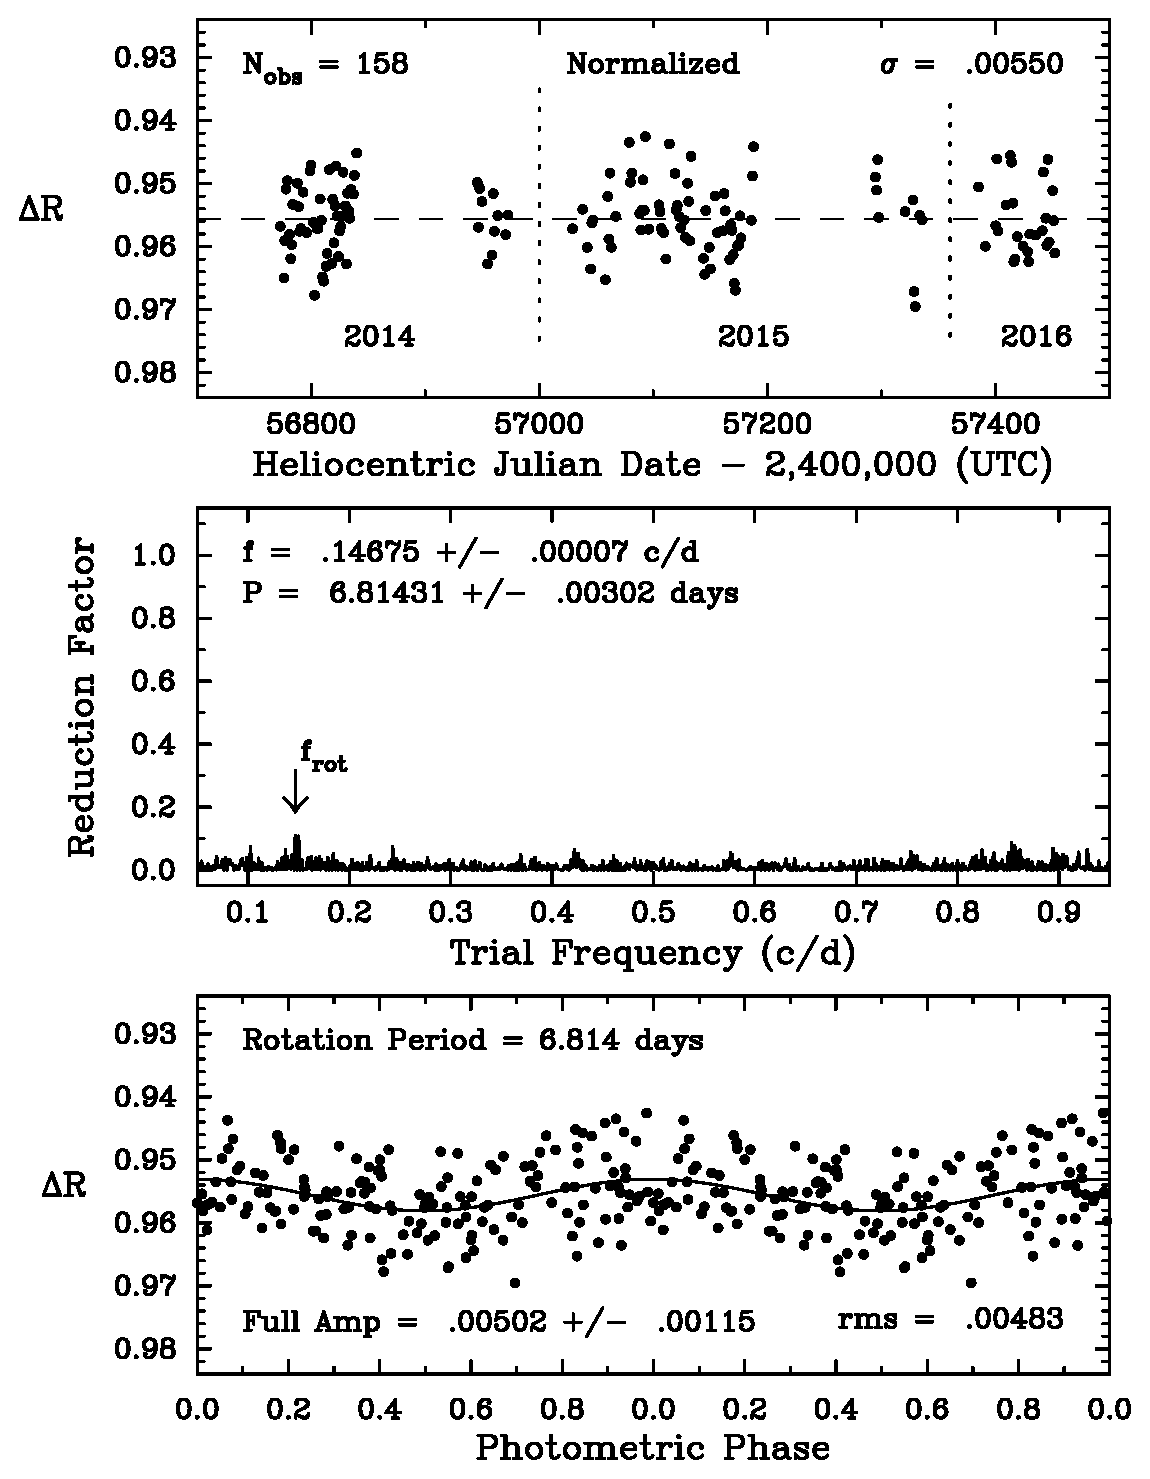
\includegraphics[width = 0.5\textwidth]{Figures/photometry.eps}
\caption{$Top$: The normalized nightly Cousins $R$ band photometric dataset for WASP-103, acquired with the C14 automated imaging telescope at Fairborn Observatory. Vertical dashed lines denote separate observing seasons. Gaps are due to target visibility and the Arizona monsoon season (July - September). $Middle$: The frequency spectrum of the normalized dataset suggests low-amplitude variability with a period of 6.814~days. $Bottom$: The normalized dataset phased to the 6.814-day period, which we interpret as the stellar rotation period. A least-squares sine fit to the 6.814-day rotation period gives a peak-to-peak amplitude of just 0.005~mag.}
\label{fig:photometry}
\end{figure}

\begin{deluxetable}{ccccc}
	%\tabletypesize{\small}
	\tablenum{1}
	\tablewidth{0pt}
	\tablecaption{Photometric Observations of WASP-103}
	\tablehead{
		\colhead{Observing} & \colhead{} & \colhead{Date Range} &
	\colhead{Sigma} & \colhead{Seasonal Mean} }% \\

%		\colhead{Season} & \colhead{$N_{obs}$} & \colhead{(HJD $-$ 2,400,000)} &
%		\colhead{(mag)} & \colhead{(mag)}}%   \\

	%	\colhead{(1)} & \colhead{(2)} & \colhead{(3)} &
	%	\colhead{(4)} & \colhead{(5)}  
	\startdata
	   2014   &  59 & 56722--56972 & 0.0057 & $0.9546\pm0.0007$  \\
	   2015   &  73 & 57028--57335 & 0.0062 & $0.9549\pm0.0007$  \\
	   2016   &  26 & 57385--57451 & 0.0055 & $0.9485\pm0.0011$  \\
	\enddata
	\label{tab:photometry}
\end{deluxetable}


\section{Light Curve Fits}
We fit a two-component model to the light curves. One component models the astrophysical signal (the planet's thermal phase variation and transit), and the other component models the systematic noise introduced by time-dependent changes in instrument performance. For each light curve, we fit the physical and systematic components simultaneously, such that the total observed flux as a function of time is given by $F(t) = F_\mathrm{physical}(t) \times F_\mathrm{sys}(t)$. For the \HST\ data, where we observed two phase curves and two additional eclipses, we constrain the physical parameters to be the same for all visits, but allow some of the systematics parameters to vary (for more details see \S\,\ref{sec:hst_sys}). We fit the WFC3 band-integrated (``white" light curve"), as well as spectroscopic light curves created from 10 wavelength bins uniformly spaced at $0.05\,\mu$m intervals between $1.15$ and $1.65\,\mu$m.

\subsection{Astrophysical Signal}
We assume the measured astrophysical signal $F_\mathrm{physical}$ has the following form:
\begin{equation}
	%F_\mathrm{physical}(\lambda, t) = F_s(\lambda) (1 + \alpha(\lambda)) \times T(\lambda, t) + F_p(\lambda, t) 
	F_\mathrm{physical}(\lambda, t) =  T(\lambda, t) + c(\lambda, t) \times F_p/F_s(\lambda, t)
\end{equation}
where $T(\lambda, t)$ is the transit model (the fraction of the stellar disk that is visible at time $t$), $F_p/F_s(\lambda, t)$ is the disk-integrated planet-to-star flux, and $c$ is a correction factor for companion star dilution and the planet's tidal distortion. 

We calculated the transit model $T(t)$ with the \texttt{batman} package \citep{kreidberg15a}. Many of the physical parameters are tightly constrained by \cite{southworth15}, so we fixed the orbital period, time of inferior conjunction, orbital inclination, and ratio of semi-major axis to stellar radius to the previously published values ($P = 0.925545613$ day, $t_0 = 2456836.2964455\,\mathrm{BJD_{TDB}}$, $i = 87.3^\circ$, and $a/R_s = 2.999$). As a test, we fit for these parameters with the Spitzer Channel 2 light curve, which has the best phase coverage and least systematic noise of the three data sets. We found that the transit parameters are consistent with the \cite{southworth15} results, so we proceeded with the remainder of the analysis holding those parameters fixed.  The free parameters for the transit model were the transit depth $r_p$ and a linear limb darkening parameter $u$. 

We calculated the planet-to-star flux $F_p/F_s$ in two different ways. First, we fit a sinusoid with a period equal to the planet's orbital period. The free parameters were the sine curve amplitude and phase offset. For the second approach, we used the \texttt{SPIDERMAN} package \citep{louden17} to model $F_p/F_s$. This package allows users to input a climate map (temperature or brightness as a function of latitude and longitude), and generate the corresponding flux ratio for an observation at time $t$. In our fit, we calculated the stellar flux with a PHOENIX model \citep{husser13} interpolated to an effective temperature of $6110\,\mathrm{K}$ \citep{gillon14}.  For the planet flux, we tested three different maps: a two-temperature map, with a uniform dayside temperature $T_d$ and a uniform nightside temperature $T_n$; a map generated with spherical harmonics; and the physically-motivated kinematic model from \cite{zhang16}, which has just three free parameters (the nightside temperature $T_n$, the change in temperature from day-to-night side $\Delta_T$, and the ratio of radiative to advective timescales $\xi$).  In all cases, we assumed that the planet is tidally locked, such that each orbital revolution corresponds to one complete rotation on its spin axis. 

We scaled the planet-to-star flux by a correction factor $c$ to account for dilution from the companion star and ellipsoidal variability due to the planet's tidal distortion. The correction factor took the form: 
\begin{equation}
	c(\lambda, t) = [1 + \alpha(\lambda)]A(t)
\end{equation}
where $\alpha(\lambda)$ is the additional fractional flux from the companion star and $A(t)$ is the sky-projected area of the planet. We estimated $\alpha(\lambda)$ based on the best fit spectral energy distribution from \cite{cartier17}. The companion star contributes FIXME percent of the flux at FIXME $\mu$m.  We calculated $A(t)$ using the analytic formula from \cite{leconte11b}, equation B.9, which computes the projected area of a triaxial ellipsoid. We estimated the ellipsoid properties using Table B.3 of \cite{leconte11a}, assuming the planet radius is 1.5 $R_\mathrm{Jup}$ and age is 5 Gyr. The predicted ellipsoidal variability is shown in Figure\,\ref{fig:ellipsoidal}. At quadrature, the projected radius is $8\%$ larger than at phase zero (mid-transit). %FIXME: say this doesn't matter.
%In addition to temperature, the planet's visible surface area $[R(t)]^2$ is also expected to vary with orbital phase due to tidal distortion \citep{gillon14}. In the observed light curve, changes in planet radius are degenerate with changes in temperature. 

%We explored adding an additional sine term to model the thermal phase variation, but the additional degrees of freedom are not justified according to the Bayesian Information Criterion (BIC). 


%Our light curves are not precise enough to detect the ellipsoidal variability, but we include a model prediction $E(t)$ to avoid introducing any bias in the thermal phase variation. We model $E(t)$ using the analytic expression from \cite{leconte11}, which 
%FIXME doppler beaming?

\begin{figure}
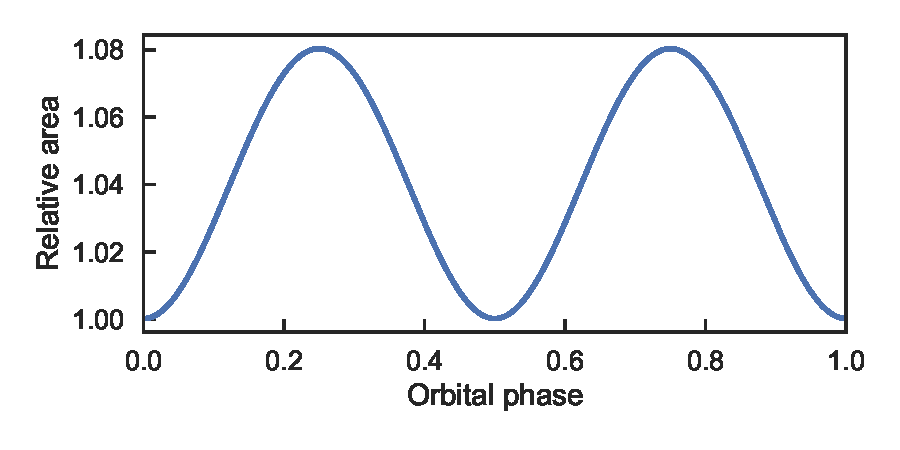
\includegraphics[width = 0.5\textwidth]{Figures/ellipsoidal.pdf}
\caption{Projected area of the planet as a function of orbital phase, normalized to unity at phase zero. The area variation was predicted analytically using the model from \cite{leconte11b}.}
\label{fig:ellipsoidal}
\end{figure}

\begin{figure}
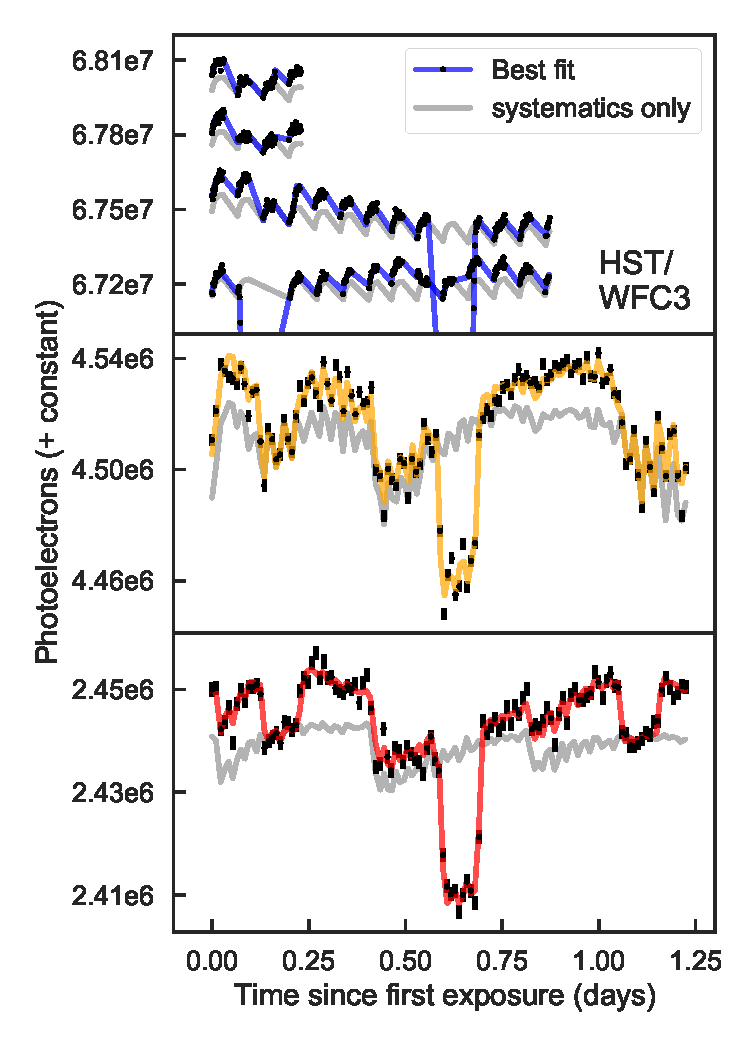
\includegraphics[width = 0.5\textwidth]{Figures/systematics.pdf}
\caption{Raw light curves for WASP-103b observed with \HST/WFC3 (top panel) and \Spitzer/IRAC (bottom two panels). The data points are indicated with black dots. The \HST\ data are unbinned, and the Spitzer data are binned in time segments of FIXME minutes with error bars indicating the bin standard deviation. The colored lines show the best fit models, which include the astrophysical signal and instrument systematics. The gray lines indicate the contribution from the instrument systematics alone (which would be observed for a source with constant brightness and no planet). For visual clarity, we corrected the \HST\ data for the upstream-downstream effect, separated the four visits by adding a flux offset, and zoomed in on the phase variation, so the transits are not displayed in the panel.}
\label{fig:systematics}
\end{figure}


\subsection{Systematics}
Both the \HST\ and \Spitzer\ phase curves have systematic noise caused by variations in the sensitivity of the instrument over time. For the \HST/WFC3 data, the dominant systematic is an orbit-long exponential trend due to charge traps filling up over successive exposures \citep{long15, zhu17}. For \Spitzer\, the primary source of noise is the intrapixel sensitivity effect. The detector's pixels do not have uniform sensitivity, so slight changes in telescope pointing cause the recorded flux to vary. In Figure\,\ref{fig:systematics}, we show the raw light curves before systematic noise was removed. The systematics have comparable amplitude to the thermal phase variation signal, so they must be carefully corrected to recover the underlying planet-to-star flux. 

\subsubsection{\HST\ Systematics}
\label{sec:hst_sys}
We fit the WFC3 systematics using an analytic model of the form:
\begin{equation}
 F_\mathrm{sys}(t) = (c\,S(t) + v_1\,t_\mathrm{v} + v_2\,t_\mathrm{v}^2)(1 - \exp(-a\,t_\mathrm{orb} - b))
\end{equation}
where $t_\mathrm{v}$ is time elapsed since the first exposure in a visit and $t_\mathrm{orb}$ is time since the first exposure in an orbit. $S(t)$ is a scale factor equal to 1 for exposures with spatial scanning in the forward direction and $s$ for reverse scans, to account for the upstream-downstream effect (FIXME). The orbit-long ramp parameters are consistent for all the visits, so we constrained $a$, $b$, and $s$ to have the same value for all visits in the final fit. The visit-long trends differ from visit to visit, so $c$, $v_1$, and $v_2$ were allowed to vary between visits. We fixed $v_2$ to zero for the two secondary eclipse observations from Program 13360, since the visit-long trend for shorter observations is fit well by a linear slope.

Some segments of the data exhibit stronger systematics than others, so we exclude these data in our final analysis. We drop the first orbit from every visit and the first exposure from every orbit \citep[following common practice; see e.g.][]{kreidberg14a}.  We also discard exposures from the last half of orbit 15 from the phase curve observations, which were taken in staring mode to enable a gyro bias update. Since we observed two phase curves, we have complete orbital phase coverage the planet despite discarding some data.

\subsubsection{\Spitzer\ Systematics}
We fit the \Spitzer\ systematics with the POET pipeline, which uses the BLISS mapping technique \citep{stevenson12}. This approach creates a map of the intrapixel sensitivity while simultaneously fitting for other systematics and the physical parameters of the system. The sensitivity map is determined by bilinear interpolation over a grid of knots centered on the stellar flux. Each knot's sensitivity is calculated from the residuals to the light curve fit: the higher the flux values for data points near a given knot, the higher the detector sensitivity is at that position.  To avoid overfitting, we chose the grid scale such that bilinear interpolation performed better than nearest neighbor interpolation. For the $3.6\,\mu$m data, the grid scale was 0.008 pixel in both $x$ and $y$. For $4.5\,\mu$m, the scale was 0.022 pixel.  

In addition to the intrapixel sensitivity variation, we fit the data for a linear trend in time. We tested a quadratic trend but did not find significant evidence for the additional model complexity based on the Bayesisan information criterion (BIC). 


\begin{figure*}
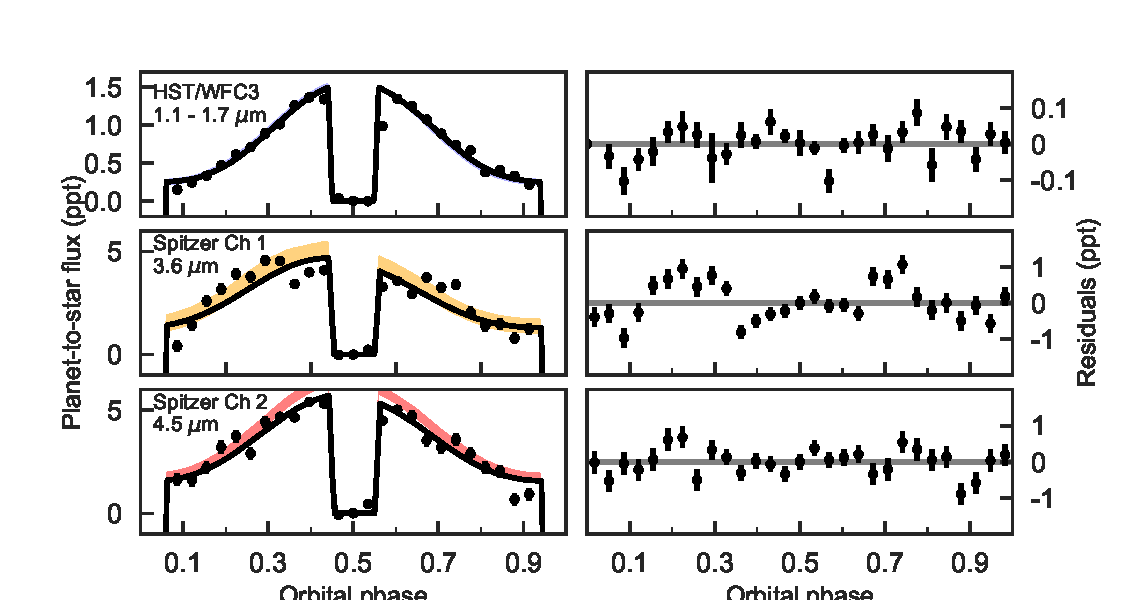
\includegraphics[width = 1.0\textwidth]{Figures/phase_curves.pdf}
\caption{WASP-103b phase curve observations from \HST/WFC3 (top) and \Spitzer/IRAC (middle and bottom). For clarity, the data are phase-folded on the planet's orbital period and binned in 30 uniformly spaced bins between 0 and 1. The left column shows the phase curves with systematic noise removed (black points) compared to the best fit model (black line). The shading denotes the  1\,$\sigma$ confidence interval on the best fit. We include the transits in the fit, but they are not displayed in this figure. The right-hand column shows the binned residuals for the best-fit light curve.}
\label{fig:phasecurves}
\end{figure*}

\section{Results}
The fitted light curves are shown in Figure\,\ref{fig:phasecurves}. This figure shows results from the kinematic model for the thermal phase variation and has instrument systematics removed.  The peak planet-to-star flux ranges from 1.5 parts-per-thousand (ppt) in the WFC3 bandpass to 5 ppt in \Spitzer Channel 2.  The planet flux changes significantly with orbital phase in all three of the data sets, suggesting a strong gradient from dayside to nightside temperature. The peak brightness occurs near phase 0.5.

\subsection{Goodness of Fit}
We performed several tests of the quality of the light curve fits.  First we predicted the level of scatter in the light curves based on photon and read noise, then compared this value to the root-mean-square (rms) of the fit residuals. The fit rms was within FIXME percent of the expected noise level in the WFC3 spectroscopic light curves and \Spitzer\ Channel 2 (expected rms of 450 and FIXME ppm). The 

Second, we tested whether the fit rms decreases as expected when the light curve in binned in time.  If the noise is ``white" (uncorrelated in time), the residuals are expected to decrease by a factor of $\sqrt{N}$, where $N$ is the number of points in a bin. Figure\,\ref{fig:rms} shows the binned residuals compared to expectations for white noise. The \HST/WFC3 and \Spitzer\ Channel 2 light curves agree well with expectations, whereas \Spitzer\ Channel 1 shows higher noise than expected as bin size increases. This test confirms the presence of time-correlated noise in the Channel 1 light curve that can be seen by eye in the residuals in Figure\,\ref{fig:phasecurves}. Both \Spitzer\ channels use the same detector, but Channel 1 data are more susceptible to time-correlated noise because the the point spread function is narrower at shorter wavelengths, making intrapixel sensitivity variations more pronounced.

The reduced $\chi^2$ values for the fits are near unity. FIXME when you have them all.
%Third, we calculated several goodness of fit statistics. $\chi^2$, AIC, BIC.

\begin{figure}
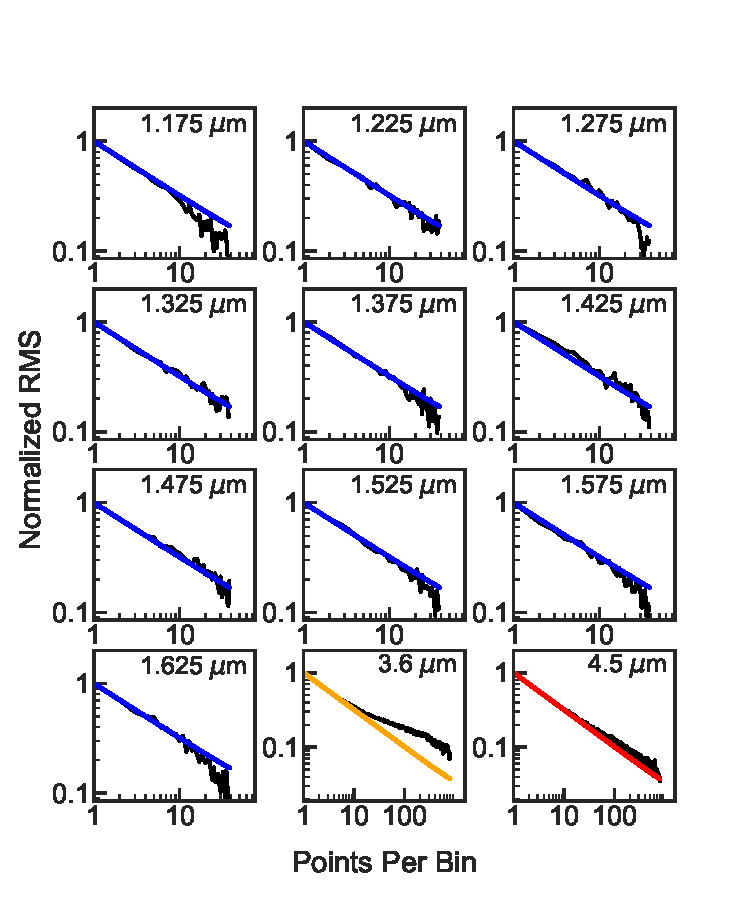
\includegraphics[width = 0.5\textwidth]{Figures/rms.pdf}
\caption{Root mean square (rms) variability in the light curves as a function of bin size (black lines) compared to the expected rms from photon noise (colored lines). The central wavelength of the light curve is indicated in the upper right corner of each panel. With the exception of the \Spitzer\ 3.6 $\mu$m channel, the rms for the light curves bins down in agreement with predictions from the photon noise.}
\label{fig:rms}
\end{figure}

\begin{deluxetable}{llllll}
	\tablecolumns{6}
	\tablewidth{0pt}:
	\tablecaption{Model Comparison \label{table:models}}
	\tablehead{
	\colhead{Data} & \colhead{Model} & \colhead{$T_\mathrm{min}$} & \colhead{$T_\mathrm{max}$} & \colhead{$\Delta_\mathrm{AIC}$} & \colhead{$\Delta_\mathrm{BIC}$}}
		\startdata
		WFC3 & Sph. Harmonics & 1214 & 3251 & 0.0 & 0.0 \\
		\, & Kinematic & 1980 & 3958 & 11.8 & 11.8 \\
		\, & Two Temp. & 0 & 2887 & 47.7 & 43.2 \\
		\, & Sinusoid & -- & -- & 17.7 & 13.2 \\
		Ch 1 & Sph. Harmonics & 1280 & 3444 & 48.0 & 0.0 \\
		\, & Kinematic & 1955 & 3675 & 82.3 & 34.3 \\
		\, & Two Temp. & 1429 & 3041 & 58.7 & 17.6 \\
		\, & Sinusoid & -- & -- & 0.0 & 98.4 \\
		Ch 2 & Sph. Harmonics & 902 & 3786 & 2.2 & 3.1 \\
		\, & Kinematic & 1703 & 4276 & 16.55 & 17.41 \\
		\, & Two Temp. & 1361 & 3311 & 26.1 & 0.0 \\
		\, & Sinusoid & -- & -- & 0.0 & 49.6 \\
		\enddata
		\vspace{-0.8cm}
		\tablecomments{comments}
\end{deluxetable}

\subsection{Phase-Resolved Spectra}
We used the best-fit phase curves (with systematics removed) to generate phase-resolved emission spectra.  Since our model does not fit eclipse depth as a free parameter, we estimated the dayside emission spectrum as follows. We used \texttt{SPIDERMAN}'s eclipse\_depth method to calculate the average planet-to-star flux for the best-fit model during secondary eclipse.  To estimate uncertainties, we took the standard deviation of the residuals of the in-eclipse data points, then added this value in quadrature to the standard deviation of the residuals of the out-of-eclipse data.  This summed error accounts for the uncertainty in the baseline flux.

For the other orbital phases, we binned the light curve (with systematics removed) in eight intervals of about 0.1 in orbital phase, with endpoints at phases $0.06, 0.15, 0.25, 0.35, 0.44$ and $0.56, 0.65, 0.75, 0.85, 0.94$. These endpoints were chosen to ensure that there is no contribution from in-transit or in-eclipse data.  In each phase bin, we estimated the planet-to-star flux from the mean value of the data points in the bin. To estimate the uncertainty, we took the standard deviation of the points in the bin and added it in quadrature to the standard deviation of the data points during secondary eclipse (phase $0.46-0.54$). This sum accounts for the uncertainty in the stellar flux (measured during secondary eclipse). The phase-resolved emission spectra are shown in Figure\,\ref{fig:spectra} and listed in Table\,\ref{table:spectra}.

To test that the phase-resolved spectra are robust to different approaches for fitting the data, we compared the spectra for all four of the thermal phase variation models (sinusoid, kinematic, spherical harmonics, and two temperature). We found that the choice of model does not significantly change the results.  The emission spectra are insensitive to the models because they are estimated directly from the data (after systematics have been removed). Since systematic noise is not strongly correlated with the thermal phase variation, the systematics-divided data are nearly identical for all the models.  This point is illustrated in Figure\,\ref{fig:model_comparison} for the broadband WFC3 light curve. In most phase bins, the planet-to-star flux agrees to well within one sigma for all the models. 

\begin{figure*}
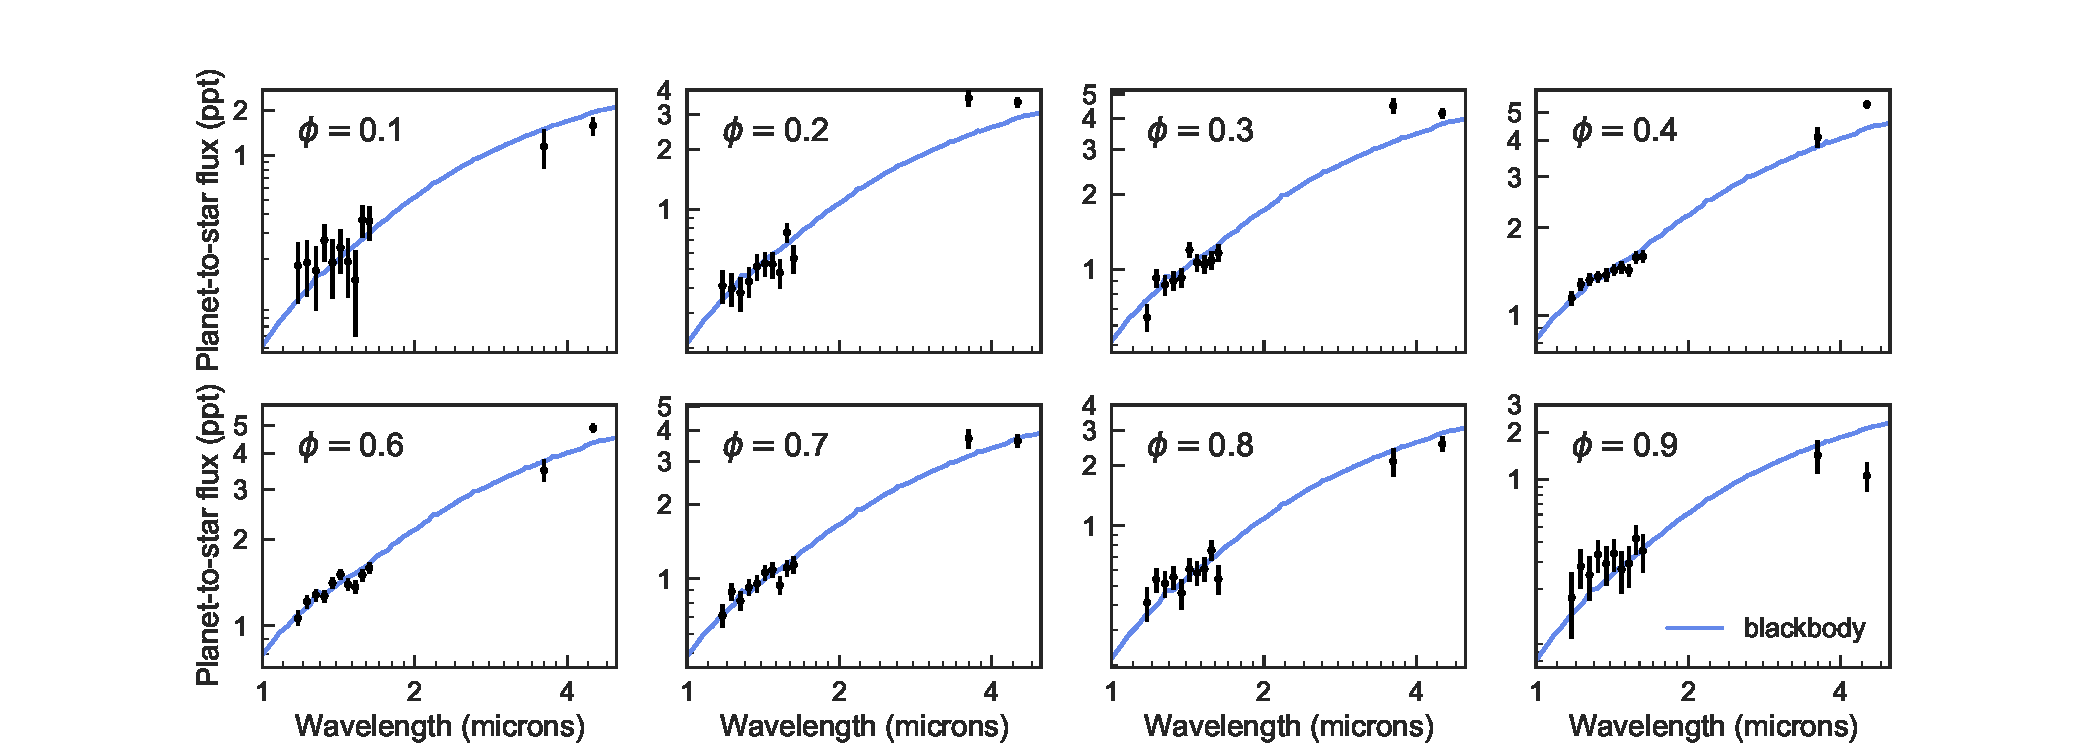
\includegraphics[width = 1.0\textwidth]{Figures/emission_spectra.pdf}
\caption{Phase-resolved emission spectra.}
\label{fig:spectra}
\end{figure*}

\begin{figure*}
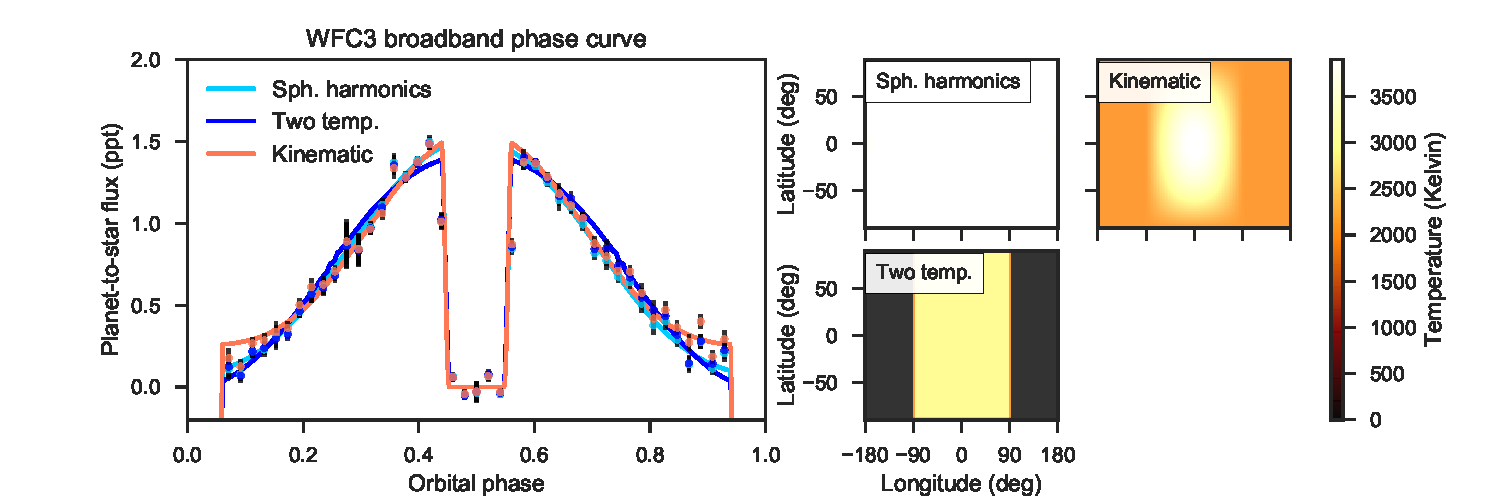
\includegraphics[width = 1.0\textwidth]{Figures/hst_model_comparison.pdf}
\caption{Left: fits to the broadband WFC3 phase curve. Right: best fit temperature maps.}
\label{fig:model_comparison}
\end{figure*}

\begin{deluxetable*}{llllllllllll}
\tablecolumns{12}
\tablewidth{0pt}:
\tablecaption{Phase-Resolved Emission Spectra \label{table:spectra}}
\tablehead{
\colhead{$\lambda$} & \colhead{Dilution} & \colhead{0.1} & \colhead{0.2} & \colhead{0.3} & \colhead{0.4} & \colhead{0.6} & \colhead{0.7} & \colhead{0.8} & \colhead{0.9} & \colhead{X} & \colhead{Y}}
\startdata
1.175 & 0.10 & $ 179 \pm 79 $ & $ 411 \pm 77 $ & $ 647 \pm 80 $ & $ 1143 \pm 65 $ & $ -15 \pm 66 $ & $ 142 \pm 67 $ & $ 1063 \pm 64 $ & $ 710 \pm 73 $ & $ 412 \pm 78 $ & $ 177 \pm 79 $ \\ 
1.225 & 0.11 & $ 188 \pm 76 $ & $ 398 \pm 74 $ & $ 928 \pm 77 $ & $ 1276 \pm 62 $ & $ 120 \pm 64 $ & $ 42 \pm 65 $ & $ 1216 \pm 62 $ & $ 888 \pm 71 $ & $ 539 \pm 75 $ & $ 280 \pm 76 $ \\ 
1.275 & 0.11 & $ 166 \pm 76 $ & $ 379 \pm 74 $ & $ 869 \pm 77 $ & $ 1323 \pm 62 $ & $ 139 \pm 64 $ & $ -8 \pm 65 $ & $ 1282 \pm 62 $ & $ 814 \pm 71 $ & $ 515 \pm 75 $ & $ 247 \pm 76 $ \\ 
1.325 & 0.11 & $ 266 \pm 75 $ & $ 432 \pm 73 $ & $ 904 \pm 76 $ & $ 1357 \pm 62 $ & $ 4 \pm 63 $ & $ 144 \pm 64 $ & $ 1267 \pm 61 $ & $ 925 \pm 70 $ & $ 552 \pm 74 $ & $ 333 \pm 75 $ \\ 
1.375 & 0.12 & $ 189 \pm 81 $ & $ 514 \pm 78 $ & $ 928 \pm 82 $ & $ 1376 \pm 66 $ & $ 131 \pm 67 $ & $ 52 \pm 68 $ & $ 1411 \pm 65 $ & $ 954 \pm 75 $ & $ 461 \pm 79 $ & $ 292 \pm 81 $ \\ 
1.425 & 0.13 & $ 238 \pm 79 $ & $ 532 \pm 76 $ & $ 1198 \pm 79 $ & $ 1431 \pm 64 $ & $ 40 \pm 66 $ & $ 185 \pm 66 $ & $ 1511 \pm 64 $ & $ 1063 \pm 73 $ & $ 605 \pm 77 $ & $ 338 \pm 79 $ \\ 
1.475 & 0.14 & $ 191 \pm 81 $ & $ 527 \pm 79 $ & $ 1068 \pm 82 $ & $ 1460 \pm 66 $ & $ 90 \pm 68 $ & $ 105 \pm 69 $ & $ 1392 \pm 66 $ & $ 1090 \pm 75 $ & $ 580 \pm 80 $ & $ 268 \pm 81 $ \\ 
1.525 & 0.14 & $ 143 \pm 84 $ & $ 478 \pm 81 $ & $ 1048 \pm 85 $ & $ 1429 \pm 69 $ & $ 103 \pm 70 $ & $ 88 \pm 71 $ & $ 1367 \pm 68 $ & $ 943 \pm 77 $ & $ 607 \pm 82 $ & $ 291 \pm 84 $ \\ 
1.575 & 0.15 & $ 367 \pm 88 $ & $ 761 \pm 85 $ & $ 1088 \pm 89 $ & $ 1581 \pm 72 $ & $ 96 \pm 73 $ & $ 125 \pm 74 $ & $ 1503 \pm 71 $ & $ 1107 \pm 81 $ & $ 754 \pm 86 $ & $ 422 \pm 88 $ \\ 
1.625 & 0.16 & $ 359 \pm 93 $ & $ 565 \pm 90 $ & $ 1169 \pm 94 $ & $ 1590 \pm 76 $ & $ 45 \pm 78 $ & $ 181 \pm 79 $ & $ 1593 \pm 75 $ & $ 1142 \pm 86 $ & $ 542 \pm 91 $ & $ 351 \pm 93 $ \\ 
3.6 & 0.17 & $ 1148 \pm 333 $ & $ 3633 \pm 330 $ & $ 4487 \pm 320 $ & $ 4107 \pm 314 $ & $ 661 \pm 324 $ & $ 373 \pm 324 $ & $ 3495 \pm 315 $ & $ 3720 \pm 330 $ & $ 2102 \pm 331 $ & $ 1431 \pm 334 $ \\ 
4.5 & 0.16 & $ 1586 \pm 220 $ & $ 3468 \pm 214 $ & $ 4188 \pm 190 $ & $ 5334 \pm 179 $ & $ 466 \pm 200 $ & $ 757 \pm 200 $ & $ 4904 \pm 183 $ & $ 3626 \pm 214 $ & $ 2575 \pm 217 $ & $ 1057 \pm 221 $ \\ 
\enddata
\vspace{-0.8cm}
\tablecomments{comments}
\end{deluxetable*}

\begin{figure}
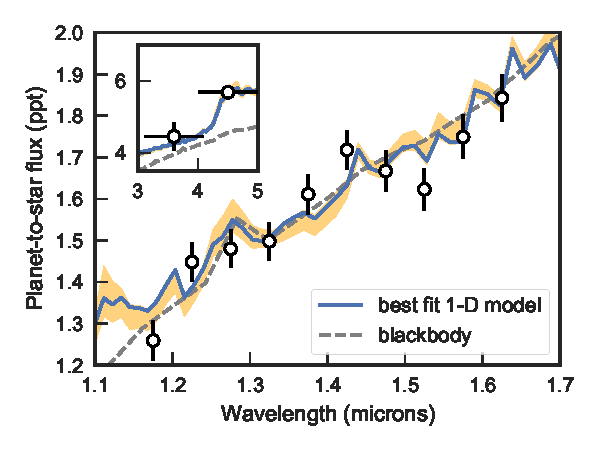
\includegraphics[width = 0.5\textwidth]{Figures/dayside_spectrum.pdf}
\caption{Dayside emission spectrum.}
\label{fig:dayside}
\end{figure}


\subsection{Comparison of Thermal Phase Variation Models}
We compared four different models for the thermal phase variation: a sinusoid and three temperature maps. The sinusoid has been the most widely used model for thermal phase variation in previous analyses of thermal phase curves \citep{FIXME} and directly fits the phase variation amplitude and offset from the substellar point. Fitting temperature maps (two-temperature, kinematic, and spherical harmonics) is a new approach enabled by the \texttt{SPIDERMAN} package.  The three maps each have different strengths: the kinematic model incorporates the most prior knowledge of physics, and even though it makes several simplifying assumptions (e.g, that the wind speed and direction are constant), it closely reproduces GCM simulations over a wide parameter space \citep{zhang16}.   The spherical harmonics map is the most flexible and makes the fewest assumptions about the true climate. The two-temperature model is the simplest and easiest to compare to one-dimensional models of the dayside, which assume a uniform temperature/pressure profile.  

All of the models provide reasonable fits to the data, with $\chi^2_\nu$ near unity, but they yield significantly different temperature maps. Table\,\ref{tab:model_comparison} lists the minimum and maximum temperatures for the best fit models to the WFC3 broadband and two Spitzer phase curves. We also list the Bayesian information criterion (BIC) and Aikike information criterion (AIC) values for the fits \citep[a $\Delta$BIC value greater than 10 constitutes strong evidence against a given model;][]{kass95}.

%Both of these statistics are an approximation of the Bayesian evidence for a given model, but the BIC penalizes model complexity relatively more than the AIC \citep{kass95}. 

The best fit model is either a sinusoid or spherical harmonics, depending on which criterion is used for model selection. The BIC generally favors the simpler spherical harmonics model because it penalizes model complexity relatively more than the AIC \citep{kass95}. The sinusoid has eight free parameters (amplitude, phase offset, eclipse duration, ingress/egress duration, and midpoint and depth for each of two eclipses), whereas the spherical harmonics model has four (for degree two).  The kinematic and two temperature models tend to perform significantly worse ($\Delta$BIC and $\Delta$AIC greater than 10).  As illustrated in Figure\,\ref{fig:model_comparison}, the kinematic model overpredicts the nightside flux, whereas the two temperature model overpredicts the flux at quadrature and underpredicts the dayside. 
%The spherical harmonics model is strongly favored for most of the data sets according to the AIC and BIC. It has slightly more free parameters than the other models (four, versus three for the kinematic model and two for the two-temperature model). 

We compared the planet's minimum and maximum temperature for the three climate maps by computing the temperatures over a $100\times100$ grid in latitude and longitude. The kinematic model has the hottest dayside temperature and the two-temperature model has the smallest. The differences in peak temperature for the models we consider ranges from $630\,\mathrm{K}$ for \Spitzer\ Channel 1 to $1070\,\mathrm{K}$ for the broadband WFC3 light curve. The minimum nightside temperature is also model-dependent: for the WFC3 data, the two-temperature model predicts a nightside temperature of zero Kelvin, whereas the best fit kinematic model has a nightside temperature of $1980\,\mathrm{K}$. %For the WFC3 data, the peak temperature ranges from $2890$ to $3960$ K, and the minimum ranges from $0$ to $1980$ K.  

These differences arise because the kinematic model allows a steep temperature gradient on the dayside, so the substellar point is much hotter than the terminator, whereas the two temperature map imposes a constant dayside temperature.  The spherical harmonics model has an intermediate temperature gradient, and fits the data the best. However, this model may not be physically realistic: on the nightside, it produces higher temperatures at the poles than at the equator, contrary to predictions from GCM (FIXME define?) simulations. 

The typical uncertainty is FIXME (run MCMC, say the systematic range is larger than the error bars). 


%The spherical harmonics model fits better according to the BIC and the AIC; however, it yields higher temperatures at the poles than at the equator, which does not agree with predictions from GCM simulations \citep{FIXME}. 

\subsection{Hotspot Offset}
The location of peak brightness of the phase curve is a proxy for the efficiency of thermal reradiation to space and relative to heat transport by advection (the radiative-to-advective timescale). The faster the reradiation, the less heat can be redistributed to the nightside. We compared the measured hotspot offset for the different models and found FIXME.

\section{Retrieval}
We performed an atmospheric retrieval to determine the composition and thermal structure of the atmosphere of WASP-103b. We used the CHIMERA retrieval suite \citep{FIXME}, as well as. Briefly, the CHIMERA model fits for the atmospheric metallicity and carbon-to-oxygen ratio, assuming the atmosphere is in thermochemical equilibrium. The temperature-pressure profile is FIXME. We included opacity from the dominant absorbing species expected at the temperatures and pressures on WASP-103b, including FIXME. Previous analyses of emission spectra of the hottest planets have not included Hminus opacity, but we find that it has a significant effect on our results. 

We also performed a simple grid search where we varied X.  

\subsection{Thermal Inversion}

\subsection{Bond Albedo}

\section{Comparison with GCMs}

\begin{figure}
	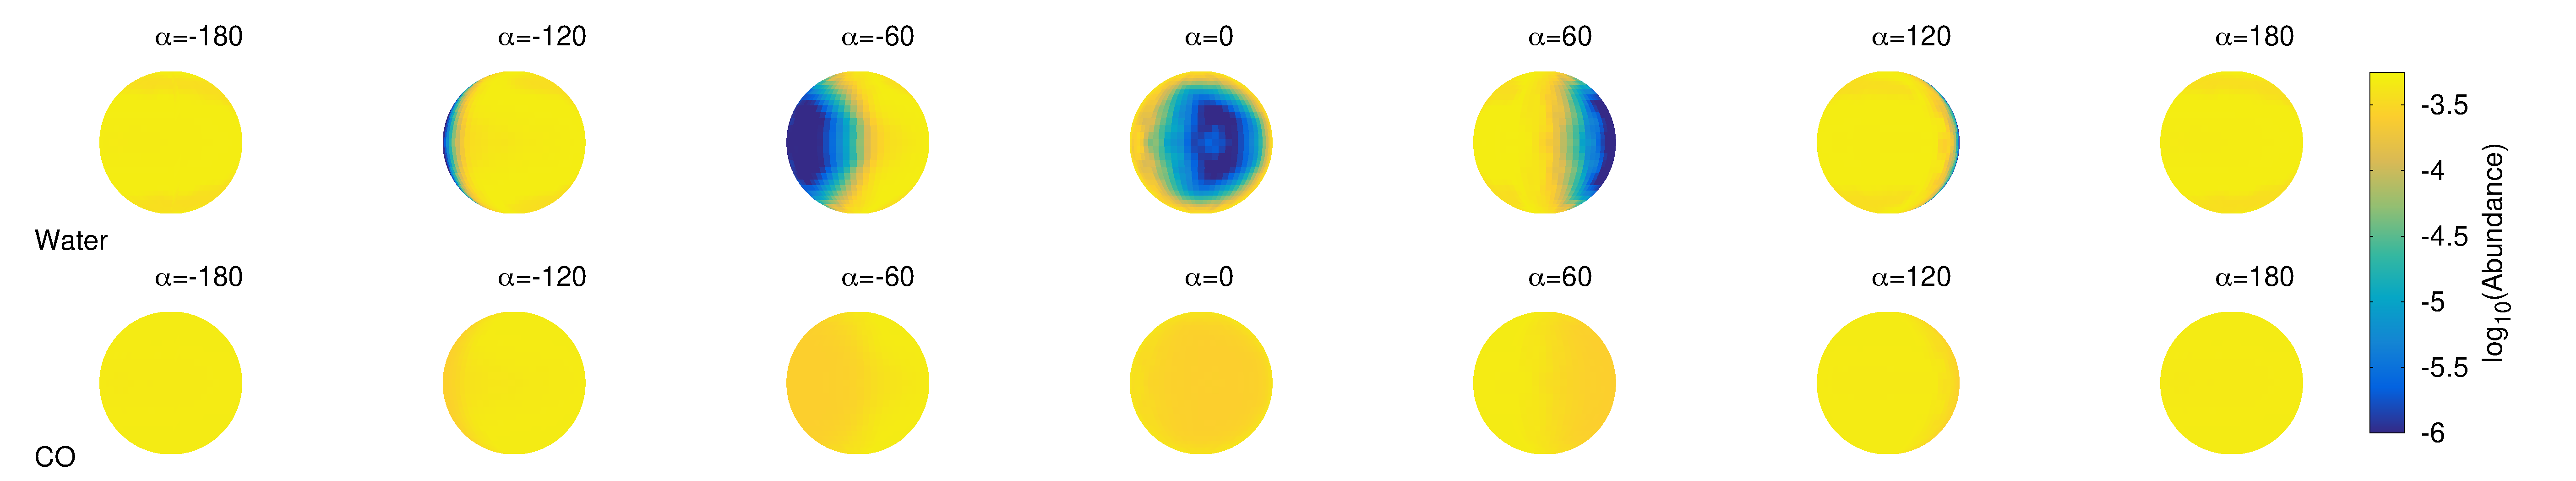
\includegraphics[width = 1.0\textwidth]{WASP-103b-Solar-NoClouds-Photo-abundances-Water-CO-4.5microns-smooth.pdf}
\caption{Water.}
\label{fig:dayside}
\end{figure}

\section{Comparison of T/P Profiles}

\section{Comparison with Brown Dwarfs and Directly Imaged Planets}
cite Tremblin et al. 2017 ? (https://arxiv.org/pdf/1710.02640.pdf)

\section{Discussion and Conclusions}

\acknowledgments
We thank a lot of people. Caroline Morley, Thomas Beatty, Ming Zhao, Kim Star Cartier, Hannah Diamond-Lowe, Nick Cowan (make him a coauthor?)

\bibliographystyle{aasjournal}
\bibliography{ms.bib}

\end{document}

